\documentclass[a4paper]{article}

%use the english line for english reports
%usepackage[english]{babel}
\usepackage[portuguese]{babel}
\usepackage[utf8]{inputenc}
\usepackage{indentfirst}
\usepackage{graphicx}
\usepackage{verbatim}


\begin{document}

\setlength{\textwidth}{16cm}
\setlength{\textheight}{22cm}

\title{\Huge\textbf{Blockade}\linebreak\linebreak\linebreak
\Large\textbf{Relatório Final}\linebreak\linebreak
\linebreak\linebreak

\includegraphics[scale=0.1]{feup-logo.png}\linebreak\linebreak
\linebreak\linebreak
\Large{Mestrado Integrado em Engenharia Informática e Computação} \linebreak\linebreak
\Large{Programação em Lógica}\linebreak
}

\author{\textbf{Grupo:}\\  João Barbosa - up201406241 \\ José Martins - up201404189 \\\linebreak\linebreak \\
 \\ Faculdade de Engenharia da Universidade do Porto \\ Rua Roberto Frias, s\/n, 4200-465 Porto, Portugal 
vspace{1cm}}
%\date{Junho de 2007}
\maketitle
\thispagestyle{empty}

%************************************************************************************************
%************************************************************************************************

\newpage

\section*{Resumo}
Resumo sucinto do trabalho com 150 a 250 palavras (problema abordado, objetivo, como foi o problema resolvido/abordado, principais resultados e conclusões).

\newpage

\tableofcontents

%************************************************************************************************
%************************************************************************************************

%*************************************************************************************************
%************************************************************************************************

\newpage

%%%%%%%%%%%%%%%%%%%%%%%%%%
\section{Introdução}


Este trabalho foi desenvolvido no âmbito da unidade curricular “Programação em Lógica” do 3º ano do Mestrado Integrado em Engenharia Informática e Computação da Faculdade de Engenharia da Universidade do Porto. O seu objetivo é o de implementar em Prolog um jogo de tabuleiro de 2 jogadores de forma a possibilitar o jogo Humano vs. Humano, Humano vs. Computador e Computador vs. Computador.
Neste relatório será descrito o jogo que escolhemos para a nossa implementação – o “Blockade” – assim como as suas regras. De seguida, serão detalhadas algumas funcionalidades e características da nossa implementação, desde a representação do jogo e visualização do tabuleiro até a avaliação de jogadas pelo computador e final do jogo. Por fim, serão apresentadas as conclusões que obtivemos da realização deste trabalho, bem como a sua bibliografia.



%%%%%%%%%%%%%%%%%%%%%%%%%%
\newpage
\section{O Jogo Blockade}

Blockade trata-se de um jogo de tabuleiro produzido pela primeira vez em 1975 pela Lakeside Games.
O jogo é desenhado para 2 jogadores sendo que cada um possui: 

\begin{itemize}
\item 2 Peões
\item 9 Parede verdes (que só podem ser colocadas verticalmente)
\item 9 Paredes azuis (que só podem ser colocadas horizontalmente)
\end{itemize}

O tabuleiro do jogo é um quadriculado com dimensões 11x14, com 2 pontos amarelos e dois pontos laranja que representam a base, e as posições iniciais, dos dois peões de cada jogador. Estes pontos distam 4 quadrículas de cada canto na diagonal. 

\begin{center}
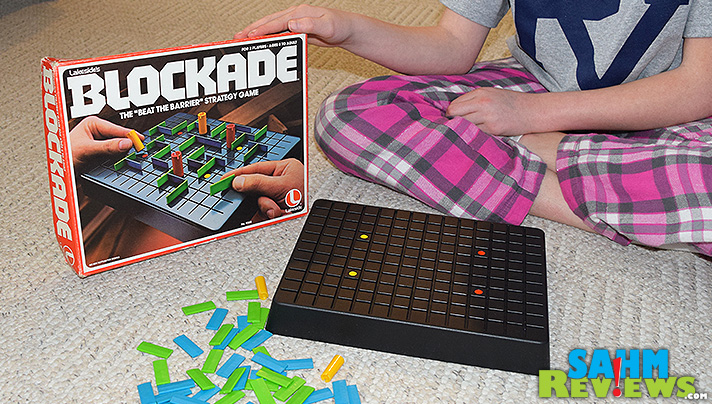
\includegraphics[scale = 0.3]{fig1.jpg}
\end{center}

Trata-se de um jogo de turnos, em que em cada turno um jogador pode mover um dos seus peões, uma ou duas quadrículas (horizontalmente, verticalmente ou uma combinação das duas), e posicionar uma parede de modo a tentar bloquear os movimentos do adversário.
As paredes ocupam sempre duas quadrículas e devem ser posicionadas de acordo com a sua cor. Peões podem saltar por cima de outros peões que estejam a bloquear o seu caminho.
O objetivo do jogo é levar um dos seus peões até à base de um dos peões do adversário. Quando os jogadores ficarem sem paredes para colocar, continuam a mover-se até que alguém vença o jogo. 

\begin{center}
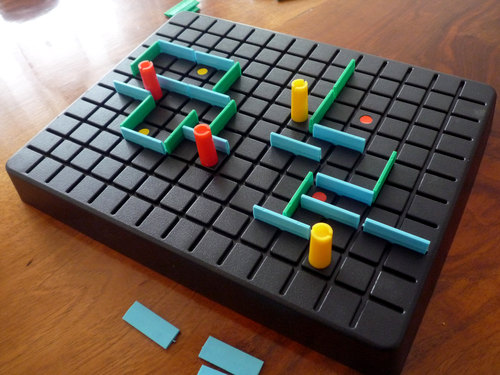
\includegraphics[scale = 0.4]{fig2.jpg}
\end{center}

%%%%%%%%%%%%%%%%%%%%%%%%%%
\section{Lógica do Jogo}


\subsection{Representação do Estado do Jogo} 

O jogo possui uma representação interna, utilizada para o processamento e armazenamento de informação, e uma representação externa, para tornar a visualização do jogo mais apelativa e intuitiva. A simbologia utilizada é a seguinte: 


\begin{center}
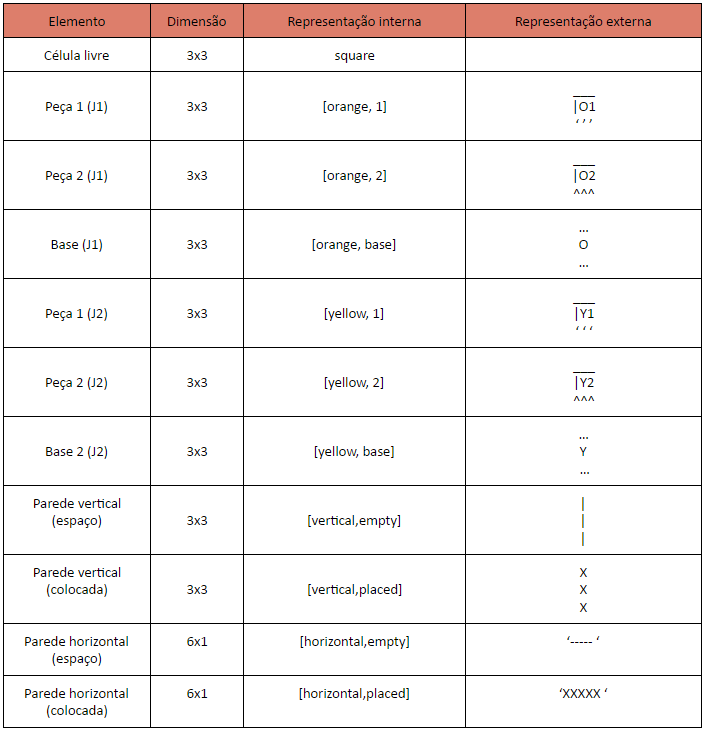
\includegraphics[scale = 0.7]{fig3.png}
\end{center}

%%%%%%%%%%%%%%%%%%%%%%%%%%
\newpage
\subsection{Visualização do Tabuleiro} 
O tabuleiro será visualizado através da utilização de caracteres ASCII para representar os peãos, paredes e bases de cada jogagor, exemplo:


\begin{center}
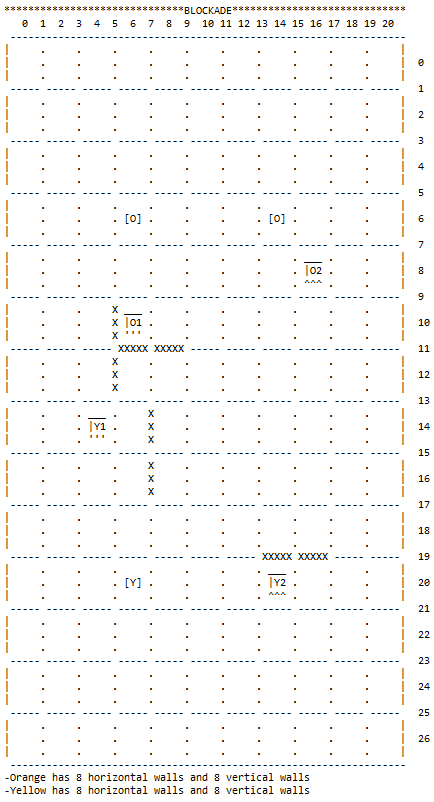
\includegraphics[scale = 0.7]{fig4.png}
\end{center}


\subsection{Lista de Jogadas Válidas} 

As jogadas são obtidas através do input do jogador ou através dos algoritmos implementados para permitir calcular a jogada do computador, sendo posteriormente verificada a sua validade.

%%%%%%%%%%%%%%%%%%%%%%%%%%
\newpage
\subsection{Execução de Jogadas} 

Depois de obtidas as coordenadas para a movimentação do jogador é utilizado o predicado validPosition(+Pawn,+ Board, +X,+ Y,-Nx,-Ny), este predicado recebe o offset (X,Y) para onde o jogador se quer mover em relação á sua posição atual e falha quando as coordenadas finais da ''futura'' posição do jogador se encontram fora das dimensões do tabuleiro ou quando existe uma parede a bloquear a movimentação para as novas coordenadas.\\
Assim que a jogada se encontra validada é chamado o predicado moveOneSpace(+Pawn, +X, +Y, +Board, -NewBoard), que move o peão num offset (X,Y) criando um novo tabuleiro.\\
Existe tambem outro predicado para validar e posicionar as paredes. Este denomina-se placeWall(+Player,+X,+ Y,+O,+Board, -NewBoard),  o predicado é bem sucedido quando as coordenadas da parede são validas, criando assim um novo tabuleiro.\\
No entanto o predicado fallha quando as coordenadas são invalidas devido a um dos motivos:
\begin{itemize}
\item A parede está para lá dos limites do tabuleiro
\item A parede está cruzada com outra parede
\item A parede bloqueia completamente o jogador (ou seja quando o posicionamente da parede impossibilita que um dos peões deixe de ter um caminho para as bases adversárias)
\end{itemize}


Validação e execução de uma jogada num tabuleiro, obtendo o novo estado do jogo. Exemplo: \textit{move(+Move, +Board, -NewBoard)}.

\subsection{Avaliação do Tabuleiro} Avaliação do estado do jogo, que permitirá comparar a aplicação das diversas jogadas disponíveis. Exemplo: \textit{value(+Board, +Player, -Value)}.

\subsection{Final do Jogo} Verificação do fim do jogo, com identificação do vencedor. Exemplo: \textit{game\_over(+Board, -Winner)}.

\subsection{Jogada do Computador} Escolha da jogada a efetuar pelo computador, dependendo do nível de dificuldade. Por exemplo: \textit{choose\_move(+Level, +Board, -Move)}.


%%%%%%%%%%%%%%%%%%%%%%%%%%
\section{Interface com o Utilizador}

Descrever o módulo de interface com o utilizador em modo de texto.


%%%%%%%%%%%%%%%%%%%%%%%%%%
\section{Conclusões}
Que conclui deste projecto? Como poderia melhorar o trabalho desenvolvido?


\clearpage
\addcontentsline{toc}{section}{Bibliografia}
\renewcommand\refname{Bibliografia}
\bibliographystyle{plain}
\bibliography{myrefs}

\newpage
\appendix
\section{Anexo Código}
Código Prolog implementado devidamente comentado e outros elementos úteis que não sejam essenciais ao relatório.

\end{document}
